\documentclass[10pt]{beamer}
\usetheme{CambridgeUS}
\usecolortheme{beaver}

\usepackage{pgfplots}
\usepackage{algorithm}
\usepackage{graphics}
\usepackage{graphicx}
\usepackage{amsmath}
\usepackage{mathtools}
\usepackage{algorithm,algorithmic}

% \addbibresourse{thesis.bib}

\begin{document}

\title[Modeling OEC using EXAFS]{Modeling Metal Protein Complexes from Experimental Extended X-ray Absorption Fine Structure using Evolutionary Algorithms}

\author[Price]{
	Collin Price
	\\
	{\small Supervisor: Sheridan Houghten}
}

% \author[Price \and Houghten \and Vassiliev \and Bruce]{
% 	Collin Price
% 	\and
% 	Sheridan Houghten
% 	\and
% 	Sergey Vassiliev
% 	\and
% 	Doug Bruce
% }
\institute{Brock University
\\
Computer Science}

\begin{frame}
	\titlepage
\end{frame}

\section{Introduction}

\begin{frame}
	\frametitle{Outline}
	\tableofcontents
\end{frame}

\begin{frame}
	\frametitle{Cofactor}

	\begin{columns}[T]
		\begin{column}{.5\textwidth}
			\begin{itemize}
				\item ``Helper'' molecules
				\item Assist in biochemical transformations
				\item Non-protein chemical compound
				\item Exist within a protein
			\end{itemize}
		\end{column}
		\begin{column}{.5\textwidth}
			\begin{figure}
				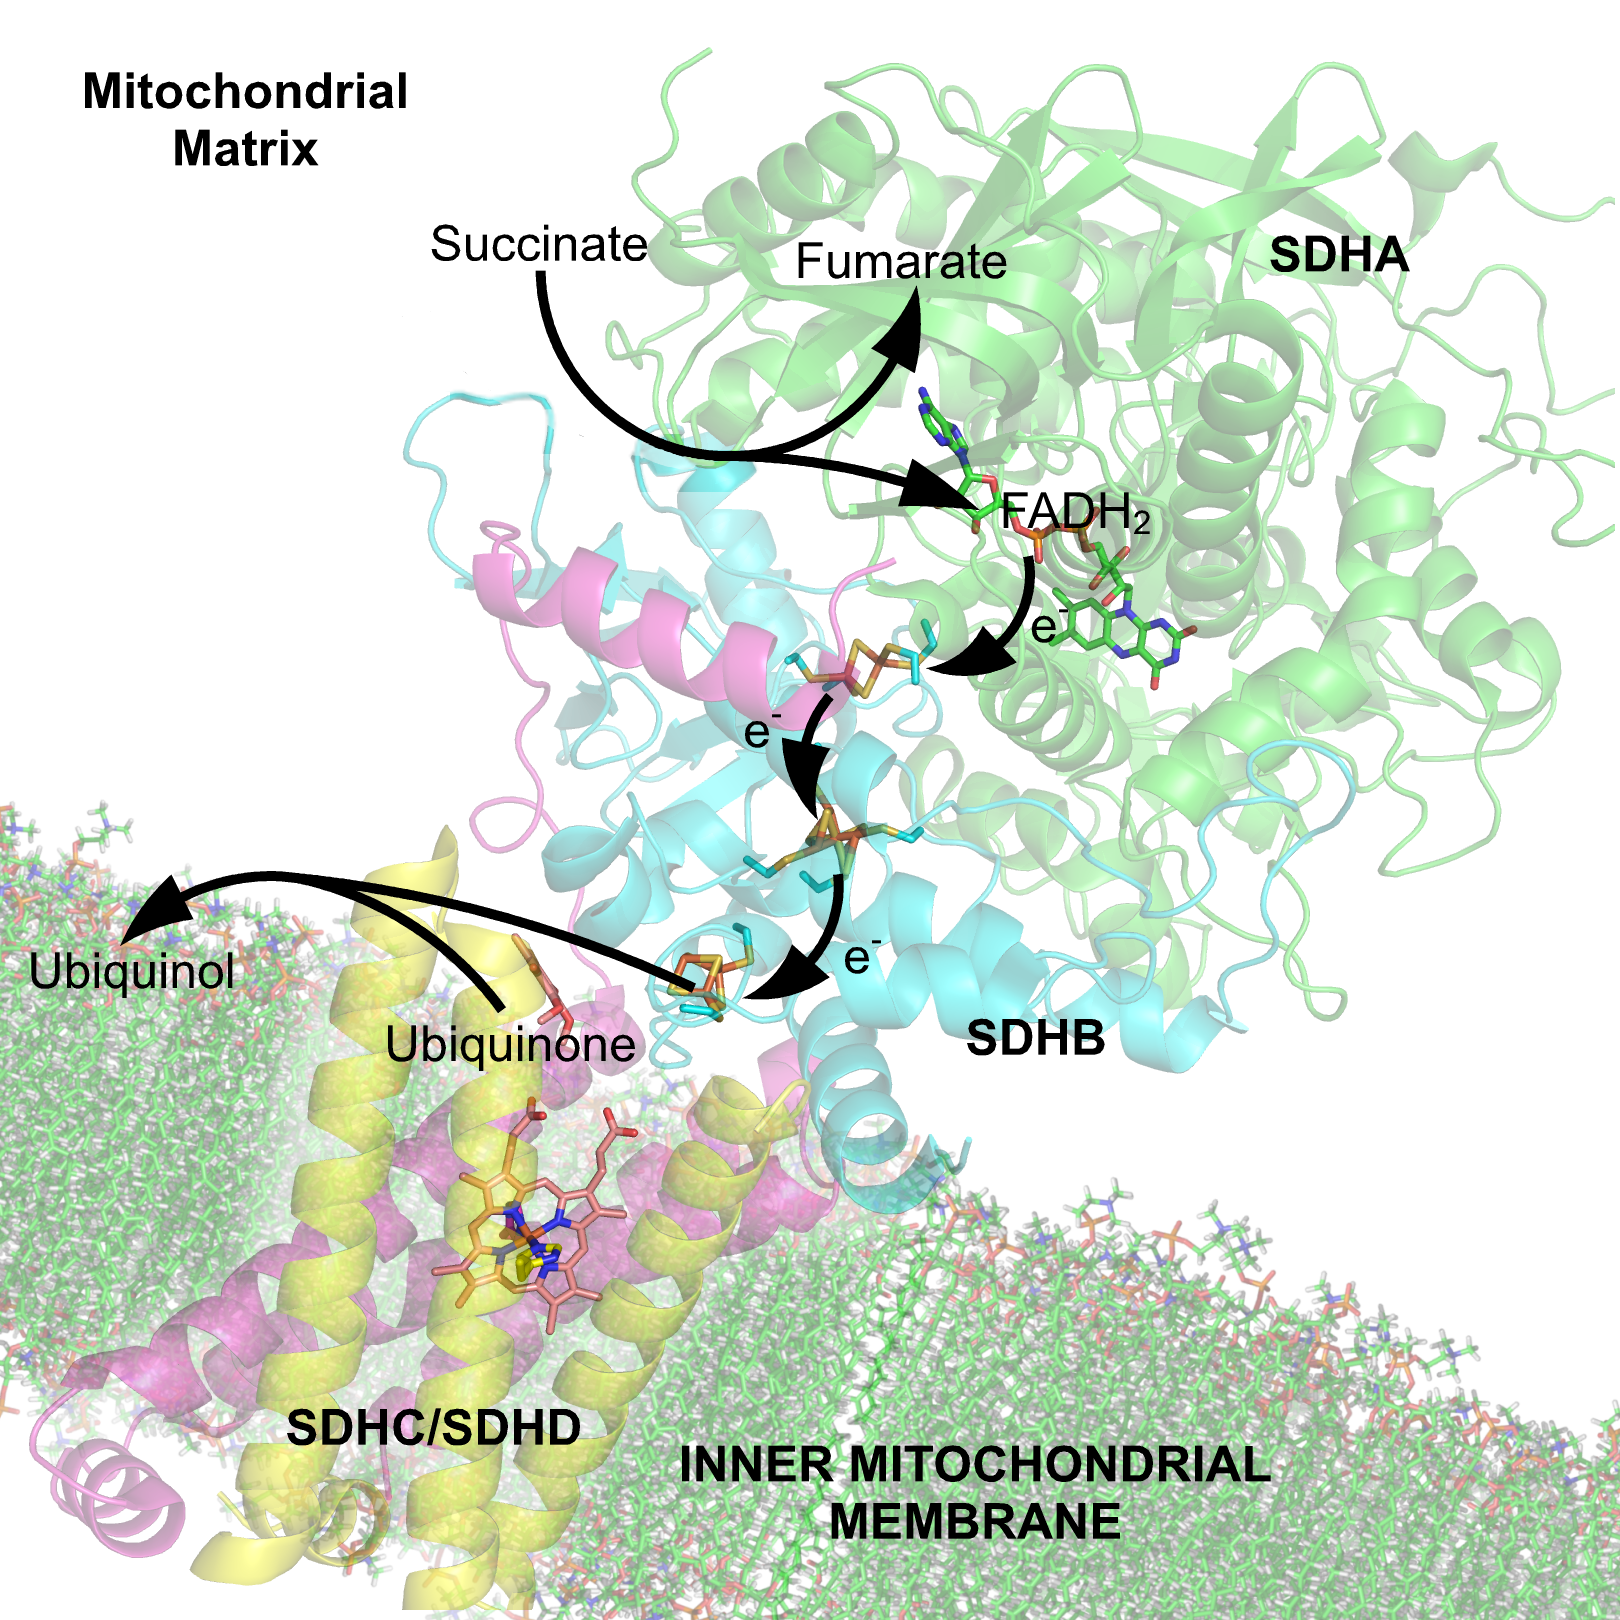
\includegraphics[width=1.0\textwidth,natwidth=1630,natheight=1620]{img/Succinate_Dehydrogenase_1YQ3_Electron_Carriers_Labeled.png}
				\caption{Cofactor Examples}
			\end{figure}
		\end{column}
	\end{columns}
	
\end{frame}

\begin{frame}
	\frametitle{Oxygen-Evolving Complex (OEC)}

	\begin{columns}[T]
		\begin{column}{.5\textwidth}
			\begin{itemize}
				\item The water-oxidizing enzyme of photosystem II.
				\item Water-splitting complex.
				\item Exists in 5 states: $S_{0}$ to $S_{4}$.
				\item Splits $H_{2}O$ into hydrogen and oxygen.
				\item $S_{4}$ reacts with water to produce oxygen.
				\item Process is not completely understood.
				\item $S_{1}$ is examined in this work.
			\end{itemize}
		\end{column}
		\begin{column}{.5\textwidth}
			\begin{figure}
				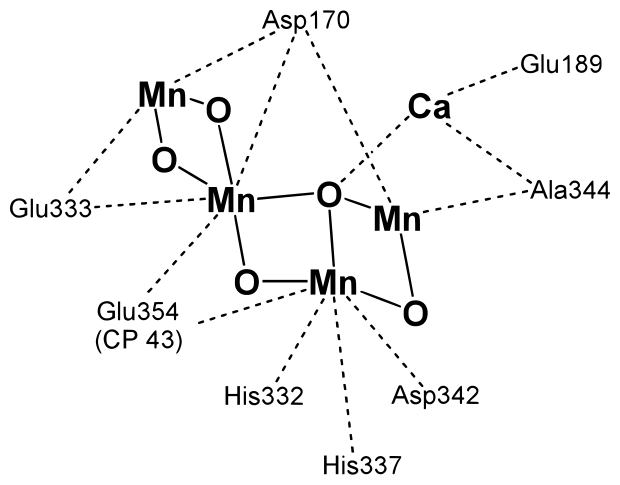
\includegraphics[width=1.0\textwidth,natwidth=620,natheight=485]{img/oec.png}
				\caption{Metalloenzyme core of the OEC}
			\end{figure}
		\end{column}
	\end{columns}

\end{frame}

\begin{frame}
	\frametitle{Experimental Extended X-ray Absorption Fine Structure (EXAFS)}
	
	\begin{itemize}
		\item A method used to measure the absorption coefficient of a material as a function of energy.
		\item X-ray is tuned to have the same wavelength as the target atom.
			\begin{itemize}
				\item In the case of the OEC we targeted the four Manganese atoms.
			\end{itemize}
		\item X-ray reacts with target atom causing the atom to lose an electron and interact with neighbouring atoms.
		\item Fluorescence energies are emitted and measured.
	\end{itemize}

\end{frame}

\begin{frame}
	\frametitle{Experimental EXAFS Spectra}

	\begin{figure}
		\begin{tikzpicture}
		  \begin{axis}[
			width=12cm,
			height=6cm,
			grid=both,
			title={EXAFS Spectra in k space},
			legend entries={Experimental},
			% legend pos=south east,
			xlabel={$k \mathbin{/} A\textsuperscript{-1}$},
			ylabel={$EXAFS \chi k\textsuperscript{3}$}
		  ]

		  \addplot[mark=x] table [col sep=comma,y index=1, x index=0] {results/best_run/for_chart.csv};

		  \end{axis}
		\end{tikzpicture}
		\caption{EXAFS Spectra of OEC in $S_{1}$}
	\end{figure}

\end{frame}

\begin{frame}
	\frametitle{Structure Refinement Problem}

	\begin{itemize}
		\item EXAFS spectra provides limited information about neighbouring atoms.
		\item We would like to know the 3-dimensional positions of each atom relative to each other.
		\item EXAFS spectra can be generated in simulations.
		\item If we match the calculated EXAFS spectra with the experimental EXAFS spectra it is likely we found the correct configuration.
		\item Goal is to minize the differences between spectra.
	\end{itemize}

\end{frame}

\begin{frame}
	\frametitle{Example Spectrum Comparison}

	\begin{figure}
		\begin{tikzpicture}
		  \begin{axis}[
			width=12cm,
			height=6cm,
			grid=both,
			title={EXAFS Spectra in k space},
			legend entries={Experimental,Calculated},
			% legend pos=south east,
			xlabel={$k \mathbin{/} A\textsuperscript{-1}$},
			ylabel={$EXAFS \chi k\textsuperscript{3}$}
		  ]

		  \addplot[mark=x] table [col sep=comma,y index=1, x index=0] {results/best_run/for_chart.csv};
		  \addplot[mark=*,mark size=1,color=red] table [col sep=comma,y index=2, x index=0] {results/best_run/for_chart.csv};

		  \end{axis}
		\end{tikzpicture}
		\caption{OEC EXAFS Spectrum Comparison}
	\end{figure}

\end{frame}

\section{Previous Work}

\begin{frame}
	\frametitle{Previous Work}

	\begin{itemize}
		\item A model of the oxygen-evolving center of photosystem II predicted by structural refinement based on EXAFS simulations
			\begin{itemize}
				\item \textit{Sproviero, Eduardo M and Gasc{\'o}n, Jos{\'e} A and McEvoy, James P and Brudvig, Gary W and Batista, Victor S}
			\end{itemize}
		\item $S_{1}$-state model of the $O_{2}$-evolving complex of photosystem II
			\begin{itemize}
				\item \textit{Luber, Sandra and Rivalta, Ivan and Umena, Yasufumi and Kawakami, Keisuke and Shen, Jian-Ren and Kamiya, Nobuo and Brudvig, Gary W and Batista, Victor S}
			\end{itemize}
		\item Density functional theory quantum mechanics and molecular mechanics hybrid (DFT-QM/MM)
		\item Monte Carlo method (R-QM/MM)
		\item Previous techniques would converge on local minima.
	\end{itemize}

\end{frame}

\section{Experiments}

\subsection{Genetic Algorithm and Restarting Genetic Algorithm}

\begin{frame}
	\frametitle{Genetic Algorithm (GA)}

	\begin{itemize}
		\item Shown success in past studies in finding low-energy protein conformations.
		\item Higher potential of avoiding local optima.
		\item Algorithm is able to produce a population of candidate solutions for future examination.
	\end{itemize}

\end{frame}

\begin{frame}
	\frametitle{Restarting Genetic Algorithm (RGA)}

	\begin{itemize}
		\item Variation of the Recentering-Restarting Genetic Algorithm.
		\item Used to maintain diversity within the population.
		\item Genetic Algorithm is run until the population has reached a set convergence rate.
		\item Duplicate individuals are removed from the population and new individuals are injected into the population.
	\end{itemize}

	\begin{algorithm}[H]
		\begin{algorithmic}[1]

		\IF{population has converged to minimum diversity}
		  \STATE remove all duplicate individuals;
		  \WHILE{population not full}
			\STATE insert random draw from generated individuals into population;
		  \ENDWHILE
		\ENDIF

		\end{algorithmic}
		\caption{Restarting the population}
	\end{algorithm}

\end{frame}

\begin{frame}
	\frametitle{Problem Encoding}

	\begin{columns}[T]
		\begin{column}{.5\textwidth}
			
			\begin{itemize}
				\item Set of 3-dimensional coordinates in space, where each position is assigned to a specific atom in the atomic structure.
				\item Entire OEC atomic structure contains 1269 atoms.
				\item EXAFS calculations only require 79 specific atoms.
				\item The units of measurement for each atom position are measured in Angstroms (\AA).
			\end{itemize}

		\end{column}
		\begin{column}{.5\textwidth}
			
			\begin{figure}
				\centering
				\begin{tabular}{ | l  l  l | }
					\hline
					X & Y & Z \\ \hline
					14.451 & -13.346 & 1.133 \\ \hline
					15.336 & -13.488 & 2.014 \\ \hline
					13.005 & -13.364 & 1.452 \\ \hline
					0.019 & 0.011 & 0.045 \\ \hline
					... & ... & ... \\ \hline
				\end{tabular}
				\caption{Representation 1}
			\end{figure}

		\end{column}
	\end{columns}
\end{frame}

\begin{frame}
	\frametitle{Population Generation}

	\begin{itemize}
		\item Initial OEC atomic structure came from the crystallographic photosystem II structure in the Protein Data Bank.
		\item Randomly moving each atom produced too many unusable configurations.
		\item Needed to generate feasible structures for starting GA population.
		\item Used a molecular dynamics simulation to obtain these structures (NAMD).
		\item Produced 10 000 atomic structures.
		\item Evaluated each atomic structure and kept the top 3\%.
	\end{itemize}
\end{frame}

\begin{frame}
	\frametitle{Operators}

	\begin{itemize}
		\item Crossover operator
			\begin{itemize}
				\item One-point crossover
				\item Least destructive to the individuals
			\end{itemize}
		\item Mutation operator
			\begin{itemize}
				\item Single atomic coordinate is randomly moved my 0.05\AA\ using Euclidean distance.
				\item Tested moving atomic coordinates by 0.001\AA, 0.005\AA, 0.01\AA, 0.025\AA, 0.05\AA, 0.1\AA, 0.5\AA, 1\AA, and 5\AA.
				\item 0.05\AA\ was chosen because it produced at least a 1\% change in fitness for all chemical elements.
			\end{itemize}
		\item Selection operator
			\begin{itemize}
				\item 3-tournament selection
			\end{itemize}
	\end{itemize}

\end{frame}

\begin{frame}
	\frametitle{Fitness}

	\begin{itemize}
		\item The goal of the experiment is to find an atomic structure that generates the same EXAFS spectrum as the experimental EXAFS spectrum.
		\item FEFF6 is used to simulate an XAFS experiment.
		\item IFEFFIT does post processing of the simulated EXAFS spectra.
		\item IFEFFIT was developed at CARS, the Consortium for Advanced Radiation Sources at The University of Chicago.
		\item The root-mean-square deviations (RMSD) is used to calculate the difference between the experimental and calculated EXAFS spectra.
	\end{itemize}

	\begin{equation}
		RMSD = \sqrt{\frac{\sum_{t=1}^{n} \left ( x_{1,t}-x_{2,t} \right )^{2}}{n}}
	\end{equation}

\end{frame}

\begin{frame}
	\frametitle{Example Spectrum Comparison}

	\begin{figure}
		\begin{tikzpicture}
		  \begin{axis}[
			width=12cm,
			height=6cm,
			grid=both,
			title={EXAFS Spectra in k space},
			legend entries={Experimental,Calculated},
			% legend pos=south east,
			xlabel={$k \mathbin{/} A\textsuperscript{-1}$},
			ylabel={$EXAFS \chi k\textsuperscript{3}$}
		  ]

		  \addplot[mark=x] table [col sep=comma,y index=1, x index=0] {results/best_run/for_chart.csv};
		  \addplot[mark=*,mark size=1,color=red] table [col sep=comma,y index=2, x index=0] {results/best_run/for_chart.csv};

		  \end{axis}
		\end{tikzpicture}
		\caption{OEC EXAFS Spectrum Comparison}
	\end{figure}

\end{frame}

\begin{frame}
	\frametitle{Experiment Setup}

	\begin{table}
		\begin{tabular}{ | l | r | }
		  \hline
			Settings & Values \\ \hline \hline
			Runs & 30 \\ \hline
			Generations & Max. 30, Until Converged \\ \hline
			Population Size & 50 \\ \hline
			Crossover Rate & 80, 70 \\ \hline
			Mutation rate & 10, 20, 30 \\ \hline
			Elitism & True, False \\ \hline
			Number of restart attempts (RGA) & 3, 5 \\ \hline
			\shortstack{Max convergence percentage \\ before restarting (RGA)} & 5\%, 10\% \\ \hline
		\end{tabular}
		\caption{System Parameters used in GA and RGA}
	\end{table}
\end{frame}

\begin{frame}
	% \frametitle{Results from GA and RGA Experiments}

	\begin{table}
	  \small
	  \begin{tabular}{ | l | l | l | l | l | l | l | l | c | c | }
		\hline
		Gen. & Crossover & Mutation & Elitism & Best RMSD & Avg. Best RMSD \\ \hline \hline
		30 & 80\% & 20\% & False & 1.2471 & 1.3518 \\ \hline
		30 & 80\% & 10\% & False & 1.1880 & 1.3610 \\ \hline
		30 & 70\% & 30\% & False & 1.1173 & \textbf{1.2942} \\ \hline
		
		30 & 80\% & 20\% & True & 1.2287 & 1.3294 \\ \hline
		30 & 80\% & 10\% & True & 1.2349 & 1.3658 \\ \hline
		30 & 70\% & 30\% & True & \textbf{1.0533} & 1.3044 \\ \hline
	  \end{tabular}
	  \caption{Results from GA Experiments}
	\end{table}

	\begin{table}
	  \small
	  \begin{tabular}{ | l | l | l | l | l | l | l | l | l | l | }
		\hline
		Gen. & Xover & Mut. & Elitism & Conv. Rate & Restarting & Best & Avg. Best \\ \hline \hline
		61 & 80\% & 20\% & True & 10\% & 3 & 1.1297 & 1.2532 \\ \hline%1
		73 & 80\% & 20\% & True & 5\% & 3 & 1.1174 & 1.2468 \\ \hline%2
		86 & 80\% & 20\% & True & 10\% & 5 & 1.0388 & 1.2252 \\ \hline%3
		106 & 80\% & 20\% & True & 5\% & 5 & \textbf{0.9649} & 1.2149 \\ \hline%4

		72 & 70\% & 30\% & True & 10\% & 3 & 1.1170 & 1.2229 \\ \hline%5
		83 & 70\% & 30\% & True & 5\% & 3 & 1.0012 & 1.2119 \\ \hline%6
		100 & 70\% & 30\% & True & 10\% & 5 & 1.0353 & \textbf{1.1808} \\ \hline%7
		133 & 70\% & 30\% & True & 5\% & 5 & 0.9992 & 1.1856 \\ \hline%8
	  \end{tabular}
	  \caption{Results from RGA Experiments}
	\end{table}

\end{frame}

\begin{frame}
	\frametitle{Analysis}

	Genetic Algorithm

	\begin{itemize}
		\item Mann-Whitney U tests performed.
		\item Experiments using a crossover rate of 70\% and a mutation rate of 30\% performed statistically better than others.
		\item May indicate problem prefers exploration over exploitation.
		\item Results show GA experiments converging early on local optima.
	\end{itemize}

	Restarting Genetic Algorithm
	
	\begin{itemize}
		\item Mann-Whitney U tests performed.
		\item RGA experiments performed statistically better than all GA experiments.
		\item Experiment with the highest number of restarts and lowest convergence criteria performed statistically better than others.
	\end{itemize}

\end{frame}

\begin{frame}
	\frametitle{Best RGA Spectrum}

	\begin{figure}
		\begin{tikzpicture}
		  \begin{axis}[
			width=12cm,
			height=6cm,
			grid=both,
			title={EXAFS Spectra in k space},
			legend entries={Experimental,Calculated},
			% legend pos=south east,
			xlabel={$k \mathbin{/} A\textsuperscript{-1}$},
			ylabel={$EXAFS \chi k\textsuperscript{3}$}
		  ]

		  \addplot[mark=x] table [col sep=comma,y index=1, x index=0] {results/best_run/for_chart.csv};
		  \addplot[mark=*,mark size=1,color=red] table [col sep=comma,y index=2, x index=0] {results/best_run/for_chart.csv};

		  \end{axis}
		\end{tikzpicture}
		\caption{OEC EXAFS Spectrum Comparison}
	\end{figure}

\end{frame}

\begin{frame}
	\frametitle{Results}

	\begin{figure}
		\begin{tikzpicture}
		  \begin{axis}[
			grid=both,
			title={Best RGA Run},
			legend entries={Best,Average},
			xlabel={Generations},
			ylabel={RMSD}
		  ]

		  \addplot[mark=x,color=red] table [col sep=comma,y index=1, x index=0] {results/best_run/results-fixed.csv};
		  \addplot[mark=*,color=blue] table [col sep=comma,y index=2, x index=0] {results/best_run/results-fixed.csv};

		  \end{axis}
		\end{tikzpicture}
		\caption{Example of a Restarting Genetic Algorithm}
	\end{figure}

\end{frame}

\subsection{Post-Optimization: Differential Evolution and Particle Swarm Optimization}

\begin{frame}
	\frametitle{Post-Optimization}

	\begin{itemize}
		\item Results from GA and RGA were successful but we could do better.
		\item Convinced by guest speaker to try Particle Swarm Optimization.
		\item Convinced by fellow student to try Differential Evolution.
		\item Used the computational intelligence library, CILIB.
	\end{itemize}
\end{frame}

\begin{frame}
	\frametitle{Particle Swarm Optimization (PSO) \& \,\,\,\,\,\,\,\,\,\,\,\,\,\,\,\,\,\,\,\,\,\,\,\,\,\,\,\, Differential Evolution (DE)}

	\begin{itemize}
		\item Excel in continuous space problems.
		\item Offers more fluid movement through the search space.
		\item Still gain a population of candidate solutions.
	\end{itemize}
\end{frame}

\begin{frame}
	\frametitle{Population Generation}

	\begin{itemize}
		\item Molecular dynamics simulation used for GA/RGA could not be used for PSO and DE.
		\item Initial atomic structure was taken from the best candidate solution from GA/RGA experiments.
		\item Population was generated by randomly moving atomic coordinate of each atom by $\pm$0.05\AA\ and $\pm$0.25\AA.
		\item Populations were initialized the same for both PSO and DE.
	\end{itemize}

\end{frame}

\begin{frame}
	\frametitle{Experiment Setup}

	\begin{table}
		\begin{tabular}{ | l | r | }
		  \hline
			Settings & Values \\ \hline \hline
			Runs & 30 \\ \hline
			Generations & 30 \\ \hline
			Population Size & 50 \\ \hline
			Initial Movement Radius & 0.05, 0.25 \\ \hline
		\end{tabular}
		\caption{System Parameters used in DE and PSO}
	\end{table}

\end{frame}

\begin{frame}
	\frametitle{Results}

	\begin{table}
		\centering
		\begin{tabular}{ | l | l | l | l | }
		  \hline
			Algorithm & Initial Movement Radius & Best RMSD & Average Best RMSD \\ \hline \hline
			DE & $\pm$0.25\AA & 1.4118 & 1.7267 \\ \hline
			PSO & $\pm$0.25\AA & 0.9296 & 1.2445 \\ \hline
			DE & $\pm$0.05\AA & 0.9973 & 1.1386 \\ \hline
			PSO & $\pm$0.05\AA & \textbf{0.7977} & \textbf{0.9001} \\ \hline
		\end{tabular}
		\caption{Results for Post-Optimization DE, and PSO}
	\end{table}

	\begin{itemize}
		\item Initial RMSD from RGA experiment was 1.0877.
		\item DE was not able to improve upon previously found candidate solutions.
		\item Lower initial movement radius performed statistically better.
		\item Post-Optimization using PSO performed statistically better RGA.
	\end{itemize}

\end{frame}

\begin{frame}
	\frametitle{Best Result: Post-Optimization PSO vs. RGA}

	\begin{figure}
		\begin{tikzpicture}
			\begin{axis}[
				width=12cm,
				height=6cm,
				grid=both,
				title={EXAFS Spectra in k space},
				legend entries={Experimental, RGA, PSO},
				legend pos=south west,
				xlabel={$k \mathbin{/} A\textsuperscript{-1}$},
				ylabel={$EXAFS \chi k\textsuperscript{3}$}
			]

				\addplot[mark=x] table [col sep=comma,y index=2, x index=0] {results/pso_results/pso-100.csv};
				\addplot[mark=-,mark size=1,color=red] table [col sep=comma,y index=2, x index=0] {results/best_run/for_chart.csv};
				\addplot[mark=*,mark size=1,color=blue] table [col sep=comma,y index=1, x index=0] {results/pso_results/pso-100.csv};

			\end{axis}
		\end{tikzpicture}
		\caption{OEC EXAFS Spectrum Comparison for PSO Post-Optimization}
	\end{figure}

\end{frame}

\subsection{Differential Evolution and Particle Swarm Optimization}

\begin{frame}
	\frametitle{Alternative Algorithms}

	\begin{itemize}
		\item PSO performed well as a post-optimization technique.
		\item Why not compare DE, and PSO directly with GA, and RGA?
		\item Initial population for DE, and PSO experiments will be from the same pool as the GA, and RGA experiments.
	\end{itemize}
\end{frame}

\begin{frame}
	\frametitle{Experimental Setup}

	\begin{table}
		\begin{tabular}{ | l | r | }
		  \hline
			Settings & Values \\ \hline \hline
			Runs & 30 \\ \hline
			Generations & 100, 200 \\ \hline
			Population Size & 50, 100 \\ \hline
			Starting Velocity & 0.01, 0.05, 0.1 \\ \hline
		\end{tabular}
		\caption{System Parameters used in DE and PSO}
	\end{table}

\end{frame}

\begin{frame}
	\frametitle{PSO Results}

	\begin{table}
		\centering
		\begin{tabular}{ | l | l | l | l | l | }
		  \hline
			Pop. Size & Gens. & Start Velocity & Best RMSD & Avg. Best RMSD \\ \hline \hline
			50 & 100 & 0.01 & 0.7735 & 0.9136 \\ \hline
			50 & 100 & 0.05 & 0.6840 & 0.9004 \\ \hline
			50 & 100 & 0.1 & 0.7498 & 0.9049 \\ \hline
			50 & 200 & 0.01 & \textbf{0.6109} & 0.8025 \\ \hline
			50 & 200 & 0.05 & 0.6653 & 0.7907 \\ \hline
			50 & 200 & 0.1 & 0.6621 & 0.7933 \\ \hline
			100 & 100 & 0.01 & 0.7392 & 0.8775 \\ \hline
			100 & 100 & 0.05 & 0.6881 & 0.8856 \\ \hline
			100 & 100 & 0.1 & 0.7306 & 0.8836 \\ \hline
			100 & 200 & 0.01 & 0.6546 & 0.7750 \\ \hline
			100 & 200 & 0.05 & 0.6571 & \textbf{0.7714} \\ \hline
			100 & 200 & 0.1 & 0.6688 & 0.7594 \\ \hline
		\end{tabular}
		\caption{Results for PSO runs}
	\end{table}

\end{frame}

\begin{frame}
	\frametitle{DE Results}

	\begin{table}
		\centering
		\begin{tabular}{ | l | l | l | l | l | }
		  \hline
			Pop. Size & Gens. & Best RMSD & Avg. Best RMSD \\ \hline \hline
			50 & 100 & 0.9793 & 1.1120 \\ \hline
			50 & 200 & \textbf{0.9405} & \textbf{1.0540} \\ \hline
			100 & 100 & 1.0357 & 1.1453 \\ \hline
			100 & 200 & 0.9646 & 1.0624 \\ \hline
		\end{tabular}
		\caption{Results for DE runs}
	\end{table}

\end{frame}

\begin{frame}
	\frametitle{Analysis}

	\begin{itemize}
		\item Population size had no effect on the results.
		\item DE, and PSO experiments statistically performed better than RGA experiments.
		\item PSO performed statistically better than DE.
		\item Might be reaching best approximation due to errors in the EXAFS spectrum.
	\end{itemize}

\end{frame}

\begin{frame}
	\frametitle{Best PSO Result}

	\begin{figure}
		\begin{tikzpicture}
		  \begin{axis}[
			width=12cm,
			height=6cm,
			grid=both,
			title={EXAFS Spectra in k space},
			legend entries={Experimental, PSO},
			legend pos=south west,
			xlabel={$k \mathbin{/} A\textsuperscript{-1}$},
			ylabel={$EXAFS \chi k\textsuperscript{3}$}
		  ]

		  \addplot[mark=x] table [col sep=comma,y index=2, x index=0] {results/pso_results/pso-100.csv};
		  \addplot[mark=*,mark size=1,color=red] table [col sep=comma,y index=2, x index=0] {data/pso-best-exafs-comparison.csv};

		  \end{axis}
		\end{tikzpicture}
		\caption{OEC EXAFS Spectrum Comparison for PSO}
	\end{figure}

\end{frame}

\begin{frame}
	\frametitle{Final Comparison}

	\begin{table}
		\centering
		\begin{tabular}{ | l | l | l | }
			\hline
			Algorithm & Best RMSD \\ \hline
			DFT-QM/MM~\cite{luber2011s1} & 1.2679 \\ \hline
			R-QM/MM~\cite{luber2011s1} & 1.2437 \\ \hline
			GA & 1.0533 \\ \hline
			RGA & 0.9649 \\ \hline
			Post-Optimized PSO & 0.7977 \\ \hline
			DE & 0.9405 \\ \hline
			PSO & \textbf{0.6109} \\ \hline
		\end{tabular}
		\caption{Summary of Best Candidate Solutions}
	\end{table}

\end{frame}

\subsection{Subset Testing}

\begin{frame}
	\frametitle{Subset Testing}

	\begin{columns}[T]
		\begin{column}{.5\textwidth}
			\begin{itemize}
				\item Individuals contain 79 atoms.
				\item Wanted reduce the search space.
				\item Tested keeping certain chemical elements rigid during experiments.
			\end{itemize}
		\end{column}
		\begin{column}{.5\textwidth}
			\begin{table}
				\caption{Chemical Element Breakdown of OEC}
				\begin{tabular}{ | l | l | }
				  \hline
					Element & Count \\ \hline
					Mn & 4 \\ \hline
					Ca & 1 \\ \hline
					O & 26 \\ \hline
					C & 14 \\ \hline
					N & 6 \\ \hline
					H & 28 \\ \hline
					Total & 79 \\ \hline
				\end{tabular}
			\end{table}
		\end{column}
	\end{columns}

\end{frame}

\begin{frame}
	\frametitle{GA Parameters}

	\begin{table}
		\caption{GA Subset Parameters}
		\begin{tabular}{ l r }
		  \hline
			Runs & 10 \\
			Population size & 50 \\
			Crossover rate & 0.7 \\
			Mutation rate & 0.3 \\
			Elitism & True \\
			% Number of restart attempts & 5 \\
			% Max convergence percentage before restarting & 5\% \\
		  \hline
		\end{tabular}
	\end{table}

\end{frame}

\begin{frame}
	\frametitle{Results}

	\begin{table}
		\caption{Results from subsets experiments}
		\begin{tabular}{ | l | l | l | l | }
			\hline
			Flexible Atoms & Rigid Atoms & Best & Average \\ \hline \hline
			Mn, Ca, C, O, N, H & None & 1.1998 & 1.2580 \\ \hline
			Mn, Ca, C, O, N & H & \textbf{1.1697} & 1.2621 \\ \hline
			Mn, Ca, C & O, N, H & 2.4413 & N/A \\ \hline
			Mn, Ca, O & C, N, H & 1.2531 & N/A \\ \hline
			Mn, Ca, N & C, O, H & 2.4881 & N/A \\ \hline
			Mn, Ca, C, O & N, H & \textbf{1.1648} & N/A \\ \hline
			Mn, Ca, C, N & O, H & 2.5143 & 2.5649 \\ \hline
			Mn, Ca, O, N & C, H & N/A & N/A \\ \hline
			Mn, Ca & C, O, N, H & 2.4916 & 2.5088 \\ \hline
		\end{tabular}
	\end{table}

	Note: N/A means there were too many invalid solutions.

\end{frame}

\section{Conclusion and Future Work}

\begin{frame}
	\frametitle{Conclusion}

	\begin{itemize}
		\item Population based search algorithms performed well on the structure refinement problem.
		\item Algorithms operating on a continuous search space performed better.
		\item Biologist needs to verify which candidate solutions are potential solutions.
	\end{itemize}

\end{frame}

\begin{frame}
	\frametitle{Future Work}

	\begin{itemize}
		\item Perform another molecular dynamics simulation on best result found from experimentation.
		\item Incorporate force fields into the algorithms to guarantee chemically feasible atomic structures.
		\item Multi-objective optimization using RMSD and potential energy.
		\item Reduce range on EXAFS spectrum comparison.
	\end{itemize}

\end{frame}

\begin{frame}
	\frametitle{Example Spectrum Comparison}

	\begin{figure}
		\begin{tikzpicture}
		  \begin{axis}[
			width=12cm,
			height=6cm,
			grid=both,
			title={EXAFS Spectra in k space},
			legend entries={Experimental,Calculated},
			% legend pos=south east,
			xlabel={$k \mathbin{/} A\textsuperscript{-1}$},
			ylabel={$EXAFS \chi k\textsuperscript{3}$}
		  ]

		  \addplot[mark=x] table [col sep=comma,y index=1, x index=0] {results/best_run/for_chart.csv};
		  \addplot[mark=*,mark size=1,color=red] table [col sep=comma,y index=2, x index=0] {results/best_run/for_chart.csv};

		  \end{axis}
		\end{tikzpicture}
		\caption{OEC EXAFS Spectrum Comparison}
	\end{figure}

\end{frame}

\begin{frame}
	
	\begin{center}
	\Huge Thank you.
	\\
	\Huge Questions?
	\end{center}

\end{frame}

\begin{frame}
	\frametitle{Bibliography}

	\bibliographystyle{ieeetr}
	\bibliography{presentation}

\end{frame}

\end{document}